\documentclass[ngerman,inputenc]{beamer}

\usepackage{amsmath, amssymb}
\usepackage{appendix}
\usepackage{booktabs}
\usepackage{pstricks}
\usepackage[utf8]{inputenc}
\usepackage{tikz}

\usepackage{graphicx} %package to manage images
\graphicspath{{images/}}

\definecolor{darkblue}{cmyk}{1.0,0.3,0,0.5}
\definecolor{darkred}{cmyk}{0.25,1,0.1,0.1}
\definecolor{uniblau}{cmyk}{1.0,0.7,0.1,0.6}
\definecolor{unihellblau}{cmyk}{0.2,0.14,0,0}
\definecolor{unihellhellblau}{cmyk}{0.05,0.035,0,0}
\definecolor{darkerblue}{cmyk}{1.0,0.3,0,0.7}

\setbeamertemplate{headline}{
\setbeamercolor{author in head/foot}{fg=white,bg=uniblau!80}
 \hbox{%
  \begin{beamercolorbox}[wd=\paperwidth,ht=2.25ex,dp=1ex,left]{author in head/foot}%
    \usebeamerfont{author in head/foot} \hspace{3pt} \insertsection%
  \end{beamercolorbox}
  }
}

\setbeamertemplate{frametitle}
{
    \setbeamercolor{frametitle}{fg=white,bg=uniblau}
    \vspace{-0.1em}
  \begin{beamercolorbox}[wd=\paperwidth,ht=3ex,dp=2ex,left]{frametitle}%
    \usebeamerfont{frametitle}\hspace{0.7em} \textbf{\insertframetitle}%
  \end{beamercolorbox}%
}

\setbeamertemplate{footline}
{
  \leavevmode%
   \hspace{-1em}
  \hbox{%
    \setbeamercolor{author in head/foot}{fg=white,bg=uniblau!60}
  \begin{beamercolorbox}[wd=.42\paperwidth,ht=2.25ex,dp=1	ex,center]{author in head/foot}%
    \usebeamerfont{author in head/foot}\insertshortauthor~~(\insertshortinstitute)
  \end{beamercolorbox}%
  \hspace{-1em}
\setbeamercolor{title in head/foot}{fg=white,bg=uniblau!80}
  \begin{beamercolorbox}[wd=.35\paperwidth,ht=2.25ex,dp=1ex,center]{title in head/foot}%
    \usebeamerfont{title in head/foot}\insertshorttitle
  \end{beamercolorbox}%
  \hspace{-1em}
  \setbeamercolor{date in head/foot}{fg=white,bg=uniblau}
  \begin{beamercolorbox}[wd=.25\paperwidth,ht=2.25ex,dp=1ex,right]{date in head/foot}%
    \usebeamerfont{date in head/foot}\insertshortdate{}\hspace*{1em}
    \insertframenumber{} /
    \inserttotalframenumber\hspace*{2ex}
  \end{beamercolorbox}}%
  \vskip0pt%
}

\let\ueberschrift=\frametitle
\renewcommand\frametitle[1]{%
  \ueberschrift{
  \rput[l](0,0){#1}
  }
}

\usecolortheme[named=uniblau]{structure}

\title[Airbnb Oslo]{Price Predictions on Airbnb Accomodations in Oslo, Norway}
\date{21.02.2022}
\author[Freitag, Beck]{Marei Freitag, Joel Beck}
\institute[University Göttingen]{Georg-August-University of Göttingen}

% display TOC before every section and subsection without duplicates
% https://stackoverflow.com/questions/2795478/latex-beamer-prevent-showing-the-toc-at-one-occasion

\RequirePackage{ifthen}
\newboolean{sectiontoc}
\setboolean{sectiontoc}{true} % default to true

\AtBeginSection[]
{
  \ifthenelse{\boolean{sectiontoc}}{
  \begin{frame}
    \frametitle{Table of Contents}
    \tableofcontents[currentsection, currentsubsection, subsubsectionstyle={show/show/shaded/shaded}]
  \end{frame}
  }
}

\AtBeginSubsection[]
{
  \begin{frame}
    \frametitle{Table of Contents}
    \tableofcontents[currentsection, currentsubsection, subsubsectionstyle={show/show/shaded/shaded}]
  \end{frame}
}

\newcommand{\toclesssection}[1]{
  \setboolean{sectiontoc}{false}
  \section{#1}
  \setboolean{sectiontoc}{true}
}


\begin{document}

\begin{frame}
  \titlepage
\end{frame}


\begin{frame}
  \frametitle{Table of Contents}
  \tableofcontents
\end{frame}

%%%%%%%%%%%%%%%%%%%%%%%%% Kapteil 1 %%%%%%%%%%%%%%%%%%%%%%%%%

\toclesssection{1. Introduction}

\begin{frame}{Introduction}

  Aims of this work:
  \begin{itemize}
    \item Establish a deep learning approach to predict the price of an accomodation per night
    \item Focus on explainability and interpretability
  \end{itemize}
  \hspace{12pt}

  $\rightarrow$ Underlying data: provided by Airbnb, contains various information about the listings in Oslo, Norway

\end{frame}


%%%%%%%%%%%%%%%%%%%%%%%%% Kapteil 2: Methods %%%%%%%%%%%%%%%%%%%%%%%%%

\toclesssection{2. Methods}

%%% Data Preprocessing %%%
\subsection{2.1 Preprocessing}

\subsubsection{Feature Engineering}

\begin{frame}{Feature Engineering: Images}

  \begin{itemize}
    \item Use transfer learning on a pretrained CNN (ResNet18) with the first 5 images per listing as input data
    \item Added Fully Connected Network at the end containing three layers and \texttt{ReLU} activation functions to be sure the CNN is able to generalize
    \item Also implemented CNN manually as a benchmark model to compare the results
          % COMMENT: Ergebnisse des selber implementierten CNN?
  \end{itemize}

  \hspace{5pt}

  Results:
  \begin{itemize}
    \item pretrained \texttt{ResNet18} achieved a Mean Absolute Error of $579$ NOK (approx. $58$ Euros) on the Validation Set
          %null model has MAE 630 NOK without log transformation, but 569 NOK with
    \item But correlation of the CNN predictions with the true price is $0.41$
          % at least positive tendencies of the CNN predictions
  \end{itemize}

\end{frame}

\begin{frame}{Image Predictions}

  \begin{figure}[H]
    \centering
    \includegraphics[width=10cm]{cnn_examples_medium.png}
    \caption{CNN example predictions}
  \end{figure}

\end{frame}


\begin{frame}{Feature Engineering: Reviews}
  % Language and Sentiment
  \begin{itemize}
    \item Language: Detect language of each review
    \item Sentiment analysis: Get the sentiment of each review
  \end{itemize}

  \hspace{5pt}

  New features per listing:
  \begin{itemize}
    \item[1.] Number of reviews
    \item[2.] Median review length
    \item[3.] Number of different languages of the reviews as well as a list of the different languages
    \item[4.] Fraction of Norwegian and English reviews
    \item[5.] Ratio of negative reviews to the total number of reviews
  \end{itemize}

\end{frame}

\begin{frame}{Wordclouds of the Reviews}

  % Wordcloud
  \begin{figure}[t]
    \centering
    \begin{minipage}{6.7cm}
      \includegraphics[width=\columnwidth]{wordcloud_eng.png}
    \end{minipage}
    \begin{minipage}{6.7cm}
      \includegraphics[width=\columnwidth]{wordcloud_nor.png}
    \end{minipage}
    \caption{Wordclouds in English and Norwegian}
    \label{fig:wordclouds}
  \end{figure}

\end{frame}


\subsubsection{Feature Selection}

\begin{frame}{Feature Selection \& Data Cleaning}

  Feature Selection:
  \begin{itemize}
    \item[1.] Manually selected features based on background knowledge, correlation analysis and the number of missing values
      %based on three criteria: background knowledge, there exists correlation between feature and price, not too many missing values because of small dataset
    \item[2.] Adjusted these features by analyzing the results of different feature selection algorithms and fitted auxiliary linear regression % mainly focused on Principal Component Analysis and Recursive Feature Selection
  \end{itemize}

  \hspace{5pt}

  Data Cleaning:
  \begin{itemize}
    \item Converting data types
    \item Splitting text-based variables into more convenient numeric or boolean features
    \item Aggregating rare categories of categorical variables into one larger \emph{Other} group to stabilize estimation % example: property type, just one House Boat with very high price (outlier?)
    \item One-Hot encoding of categorial variables and standardization of numerical variables
  \end{itemize}

\end{frame}


%%% Models %%%

\subsection{2.2 Models}

\subsubsection{Classical Models}

\begin{frame}{Classical Models}
  % In order to get some insights, we selected four classical Machine Learning models of varying complexity from the \texttt{scikit-learn} library \citep{pedregosa2011} to serve as benchmark models for our custom Neural Net.

  \begin{itemize}
    \item[1.] \textbf{Linear Regression}: simple, well understood in terms of underlying theory and highly interpretable.
    \item[2.] \textbf{Ridge Regression}: still very interpretable with a closed form analytical solution; one hyperparameter
    \item[3.] \textbf{Random Forest}: very flexible model with many hyperparameters determining e.g. the number of regression trees and the tree depth, but can be applied to many contexts and often works 'out of the box'
    \item[4.] \textbf{Histogram-Based Gradient Boosting}: modern and fast tree-based gradient boosting algorithm; large number of tunable hyperparameters
      %, some of them similar to the Random Forest parameters, some of them more specific to the \emph{Boosting} instead of the \emph{Bagging} approach such as the learning rate.
      %Similar to the very popular \href{https://xgboost.readthedocs.io/en/stable/}{XGBoost} \citep{chen2016} and \href{https://lightgbm.readthedocs.io/en/latest/}{LightGBM} \citep{ke2017} implementations that regularly outperform deep Neural Networks in Kaggle competitions on tabular data.
  \end{itemize}

\end{frame}


\subsubsection{Neural Network}

\begin{frame}{Neural Network: Model Architecture}

  \begin{columns}
    \begin{column}{0.5\textwidth}
      \begin{itemize}
        %\item Starting from roughly $60$ input features, the network width is first blown up to $256$ features before steadily decreasing it again to a single output neuron in the final layer.
        \item linear input layer (about $60$ features)
        \item $6$ intermediary \textbf{blocks} with $64$, $128$, $256$, $128$, $64$ and $8$ output features:
              \begin{itemize}
                \item[–] residual connection
                \item[–] linear layer with BatchNorm, \texttt{ReLU} activation function and dropout
              \end{itemize}
        \item $1$ output neuron
      \end{itemize}
    \end{column}
    \begin{column}{0.5\textwidth}
      \begin{center}
        \begin{figure}
          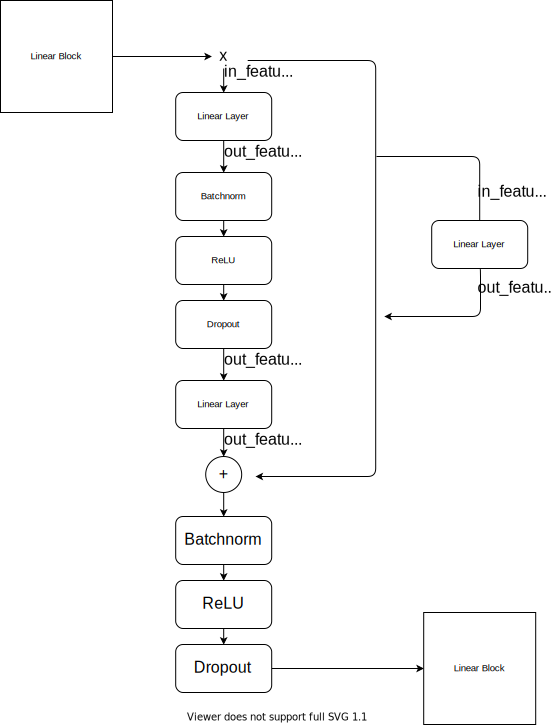
\includegraphics[width=0.9\columnwidth]{mlp_architecture.png}
          \caption{Linear Block in the FC-NN}
        \end{figure}
      \end{center}
    \end{column}
  \end{columns}

\end{frame}

\begin{frame}{Neural Network: Model Training}

  \begin{itemize}
    \item \texttt{Adam} optimizer with learning rate set to 0.01
    \item Loss function: \textit{Mean Squared Error} Loss
    \item Epochs: % COMMENT: wie viele Epochen wurden trainiert?
  \end{itemize}

  % COMMENT: hier auf den Einfluss des Dropouts eingehen?


\end{frame}




%%%%%%%%%%%%%%%%%%%%%%%%% Kapteil 3: Results %%%%%%%%%%%%%%%%%%%%%%%%%

\toclesssection{3. Results}

\subsection{3.1 Evaluation Metrics}

\begin{frame}{Evaluation Metrics}
  \begin{itemize}
    \item Mean Squared Error for \emph{Training}
    \item Mean Absolute Error and $R^2$ for \emph{Evaluation}
    \item When using log-price for model fitting, MAE and $R^2$ are computed on the \emph{original} price scale for better interpretability of the MAE
    \item Note that both metrics highly depend on the exact evaluation procedure:
          %%%
          \begin{align*}
            MAE \left(\mathbf{y}, \exp \left(\widehat{\log(\mathbf{y})}\right)\right)
             & \neq \exp \left(MAE \left(\log(\mathbf{y}), \widehat{\log(\mathbf{y})}\right) \right) \\
            R^2 \left(\mathbf{y}, \exp \left(\widehat{\log(\mathbf{y})}\right)\right)
             & \neq R^2 \left(\log(\mathbf{y}), \widehat{\log(\mathbf{y})}\right)
          \end{align*}
          %%%
    \item Direct comparisons across groups have to be taken with care
  \end{itemize}
\end{frame}

\subsection{3.2 Predictive Performance}

\begin{frame}{Training \& Validation Performance}
  \begin{figure}[h]
    \centering
    \includegraphics[width=0.8\textwidth]{model_comparison.png}
    \label{fig:model-comparison}
  \end{figure}
\end{frame}

\begin{frame}{Main Findings}
  \begin{itemize}
    \item More features tend to work better with diminishing returns ($5$ vs. all $59$ features)
    \item Classical Models: Comparable performance of linear and nonlinear models, linear models generalize better to validation set
    \item Neural Net: At first sight worst performance but best generalization
    \item The latter can be explained by differing behaviour of \emph{Dropout} and \emph{Batchnorm} layers during training and inference as well as the presence of outliers (covered later)
  \end{itemize}
\end{frame}

\begin{frame}{Main Findings}
  \begin{itemize}
    \item The price prediction task with our small tabular data does not seem to require overly complex models
    \item When including \emph{all} observations (no outlier removal) we can expect predictions within a distance of roughly $400$ NOK (40 Euros) on average to the true price and a $R^2$ value of around $0.4$.
    \item Caveat: Validation erformance is biased towards models whose hyperparameters were tuned during cross validation
  \end{itemize}
\end{frame}

\begin{frame}{Test Set Performance}
  \begin{table}[h]
    \centering
    \begin{tabular}{lrr}
      \hline
      Model                & \multicolumn{1}{c}{MAE} & \multicolumn{1}{c}{$R^2$} \\ \hline
      Linear Regression    & 404.709                 & 0.298                     \\
      Ridge                & 405.932                 & 0.294                     \\
      Random Forest        & 444.166                 & 0.268                     \\
      HistGradientBoosting & 412.243                 & 0.387                     \\
      Neural Network       & 402.24                  & 0.333                     \\
      Top2 Average         & 404.848                 & 0.296                     \\
      Top3 Average         & 399.315                 & 0.343                     \\
      Top4 Average         & 404.206                 & 0.332                     \\
      Top5 Average         & 408.116                 & 0.27                      \\ \hline
    \end{tabular}
    \caption{Test Set Performance of Classical Machine Learning Models, our custom Neural Network and Ensemble Predictions}
    \label{tab:test-set}
  \end{table}
\end{frame}

\subsection{3.3 Understanding \& Interpretation}

\subsubsection{Feature Importance}

\begin{frame}{Feature Importance}
  \begin{columns}
    \begin{column}{0.6\textwidth}
      \begin{center}
        \begin{figure}
          \includegraphics[width=\columnwidth, height=0.75\textheight]{coefficient_plot.png}
          \label{fig:coefficient-plot}
        \end{figure}
      \end{center}
    \end{column}
    \begin{column}{0.4\textwidth}
      \begin{itemize}
        \item Largest (absolute) Coefficients: \emph{room type}, \emph{property type} and \emph{neighbourhood}
        \item Top $2$ by Feature Selector: \emph{number of bedrooms} and \emph{accomodates}
        \item Marginal vs. Conditional Impact (\emph{Sentrum} neighbourhood)
      \end{itemize}
    \end{column}
  \end{columns}
\end{frame}


\subsubsection{Sensitivity to Outliers}

\begin{frame}{Impact of Outliers}
  \begin{table}[t]
    \centering
    \begin{tabular}{@{}ccc@{}}
      \toprule
      Quantile Threshold & MAE    & $R^2$ \\ \midrule
      0.0                & 443.35 & 0.16  \\
      1.0                & 337.59 & 0.51  \\
      2.5                & 282.17 & 0.53  \\
      5.0                & 240.57 & 0.54  \\
      10.0               & 214.76 & 0.49  \\ \bottomrule
    \end{tabular}
    \caption{Mean Absolute Error and $R^2$ value of the Neural Network on the validation set after removing the highest quantiles of the price distribution from the data set}
    \label{tab:mlp-outliers}
  \end{table}
\end{frame}

\begin{frame}{Impact of Outliers}
  \begin{itemize}
    \item Price outliers single most influential factor of predictive power
    \item \textbf{Not} fixed by log-transformation!
    \item Explains performance boost of Neural Network from training to validation to test set
    \item Due to different sizes and randomness, training set contains the most outliers that drive the error metrics up whereas test set contains the fewest outliers
    \item Impact diminished for classical models due to cross-validation: Extreme outliers were contained in the validation fold \emph{only once} out of multiple evaluations and metrics are averaged across all folds
  \end{itemize}
\end{frame}

\begin{frame}{Making Sense of the Data}
  \begin{itemize}
    \item Neural Net clearly lacks ability to capture entire price range accurately
    \item However, in theory the model should be flexible enough to approximate any arbitrary function reasonably well
    \item Two possible explanations:
          \begin{enumerate}
            \item The model is inherently flawed
            \item The model is faced with a nearly impossible task
          \end{enumerate}
    \item To discriminate the observations with the highest prices from the remaining ones, the corresponding feature combinations must be separable in feature space
  \end{itemize}
\end{frame}

\begin{frame}{Feature Space Embedding}
  \begin{figure}[t]
    \centering
    \includegraphics[width=0.6\textwidth]{latent_representation.png}
    \label{fig:latent-representation}
  \end{figure}
\end{frame}

\begin{frame}{Takeaways}
  \begin{itemize}
    \item Two explanations for the lack of separability:
          \begin{enumerate}
            \item The collected data is not rich or expressive enough to capture all factors that contribute to very high prices
            \item Some apartments are listed at a price that does not represent their true value
          \end{enumerate}
    \item Latter case makes entire prediction task questionable: Implicit assumption that listed prices can be justified and explained by characteristics of the joint feature distribution
    \item How to detect truly overpriced observations?
    \item Model might face expensive but fairly priced observations on new data in production \\
          $\Rightarrow$ should learn to handle those cases during training
    \item Blind removal of outliers is difficult to justify and narrows down the set of feasible target distributions!
  \end{itemize}
\end{frame}


\section{4. Munich Data}

\begin{frame}{Munich - Predictive Performance}
  \begin{itemize}
    \item About twice as large as Oslo Data \\
          $\Rightarrow$ Flexible Models like Gradient Boosting and the Neural Network benefit most
    \item However: Overall Performance \emph{not} significantly better than for Oslo Data
    \item Gradient Boosting model with best test set performance: MAE of $32.8$, $R^2$ of $0.453$
    \item Deeper/Wider architecture of neural net that is specifically designed for larger data set might lead to performance boost
  \end{itemize}
\end{frame}

\begin{frame}{Munich - Understanding \& Interpretation}
  \begin{itemize}
    \item Most important features in Linear Regression: \emph{Property Type}, \emph{Neighbourhood} and \emph{Accomodates}
    \item Munich Data again contains large price outliers with high impact on the evaluation metrics
          \vspace{1em}
          \begin{table}[h]
            \centering
            \begin{tabular}{@{}ccc@{}}
              \toprule
              Quantile Threshold & MAE   & R2   \\ \midrule
              0.0                & 42.49 & 0.31 \\
              1.0                & 35.32 & 0.44 \\
              2.5                & 30.26 & 0.42 \\
              5.0                & 25.2  & 0.45 \\
              10.0               & 22.94 & 0.4  \\ \bottomrule
            \end{tabular}
            \label{tab:munich-outliers}
          \end{table}
  \end{itemize}
\end{frame}


\section{5. Conclusion}

\begin{frame}{Conclusion}
  \begin{itemize}
    \item Linear Models show competitive predictive performance for small Oslo data
    \item Top 3 Ensemble leads to lowest test set error
    \item Large impact of outliers
    \item Possible extension to gain further understanding of the network's behaviour: \emph{Adversarial Examples} in the regression context
  \end{itemize}
\end{frame}


\begin{frame}

  \begin{center}
    \LARGE{\textbf{Thanks for listening!}}\\[10mm]
    \large{Questions?}
  \end{center}

\end{frame}


\end{document}
%